\chapter{Network layer}
\section{Routing algorithms}
\lecture{6}{12/11}

\begin{definition}[Routing]
    \textbf{Routing} is the process of selecting a path for traffic in a network or between or across multiple networks.
\end{definition}

When designing routing algorithms we must decide what to optimise, such as efficieny and fairness. We model networks as a graph of nodes and links which is updated for changes in topology (such as failures on links, or a node being down).

\begin{figure}
    \centering
    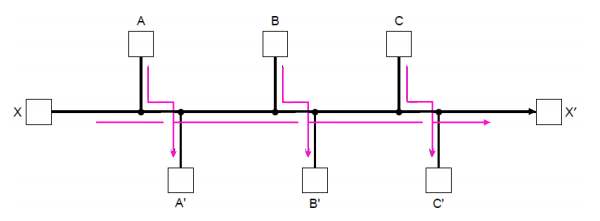
\includegraphics[width = 0.8\textwidth]{images/network-as-graph.png}
    \caption{A graph representation of a network.}
\end{figure}

\begin{proposition}[Optimality principle]
    If router $J$ is on the optimal path from $I$ to $K$, then the optimal path from $J$ to $K$ is on the same route.
\end{proposition}

\begin{definition}[Sink tree]
    A \textbf{sink tree} is a derivative graph which shows the optimal routes from all sources to a given destination.
\end{definition}

\begin{figure}
    \centering
    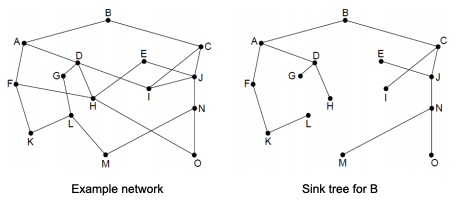
\includegraphics[width=0.8\linewidth]{images/sink-tree.png}
    \caption{A network and the sink tree for node $B$.}
\end{figure}

\begin{algorithm}[Dijsktra's]
    \textbf{Dijsktra's algorithm} computes a sink tree on the graph. Each node on the graph is labelled with its distance from the source node on the best known path. Initially no paths areknown. Each link is assigned a non-negative weight / distnace and the shortestr path is the one with the lowest total weight. More formally,
    \begin{enumerate}
        \item Start with the sink, set distance at other nodes to infinite.
        \item We have labels tenative ($\circ$) or permanent ($\cdot$), initially all tenative.
        \item Pick lowest distance non-permanent node and make it permanent.
        \item Repeat the algorithm from this node, until all nodes are permanent.
    \end{enumerate}
\end{algorithm}

This is a very well covered algorithm and should will be assumed.

We are going to move on to some dynamic routing algorithms now, of which there are two types: \emph{distance vector routing} and \emph{link state routing}.

\begin{algorithm}[Distance vector]
    Distance vector routing has the following algorithm.
    \begin{enumerate}
        \item Each node knows the dstinace of links to its immediate neighbours.
        \item Each node advertises a vector of the lowest known distances to all nodes.
        \item Each node uses received vectors to update its own.
        \item Repeat periodically.
    \end{enumerate}
\end{algorithm}

%todo example and understanding..

\begin{algorithm}[Link state routing]
    \textbf{Link state routing} is an alternative to distance vector routing. There are five steps.
    \begin{enumerate}
        \item Learn the network address of the neighbouring routers by sending \texttt{HELLO} packet, record name.
        \item Set the distance to each neighbour.
        \item Construct a packet telling all other routers what it has just learned.
        \item Send the packet to and receive packets from all other routers.
        \item Compute the shortest path with this data using Dijkstra's algorithm.
    \end{enumerate}
\end{algorithm}

\begin{definition}[Link state packet]
    In link state routing, a \textbf{link state packet} is a list corresponding to a node that lists all the node's neighbours and the weights of links to reach them.
\end{definition}

With link state routing, there is a challenge of getting these packets to \emph{all} routers. The solution to this is \emph{flooding}.

\begin{definition}[Flooding]
    \textbf{Flooding} is a method of sending a packet to all network nodes. Each node floods a new packet received on a incoming link by sending it out on all other links.
\end{definition}

It is clear that nodes must keep a track on flooded packets to avoid it happening indefinitely, but this is a good method to initial setup a routing table (as it doesn't require a routing table). 

\begin{definition}[Hierarchical routing]
    \textbf{Hierarchical routing} is a method of routing in which we divide routers into regions. In each region, we only store information about routers in that region as well as one record for every other region. 
\end{definition}

This allows for a reduced computation time when routing, but may lead to suboptimal routes being constructed.

\begin{definition}[Broadcast routing]
    \textbf{Broadcast routing} is a routing technique where upon receiving a packet, a router will flood the packet to all neighbours.
\end{definition}

This clearly will cause duplicate packets on the network, but we can use \emph{reverse path forwarding} to minimise this.

\begin{definition}[Reverse path forwarding]
    \textbf{Reverse path forwarding} is a technique in which packets that arrive at a router are checked to see if they have arrived from a preferred link (which is typically for sending packets from the source to the destination). 
\end{definition}

Although this is easy on a router's resources, it uses a large amount of a network's bandwidth and is \emph{not} a preferreed method of routing (obviously).
